\chapter{Kinematiske kurver}
\label{cha:rutherford}

I dette afsnit udledes og præsenteres de kinematiske kurver, dvs. energien som funktion af vinklen,
for hhv. Rutherfordspredning og $\alpha$-partiklen frigivet ved processen
$\Carb* \rightarrow \Be + \alpha$. Disse kurver kan ekstraheres fra data ved brug af
kalibreringsalgoritmen beskrevet i \cref{sec:kalalgo} og benyttes til at vise overensstemmelse
mellem kalibreringen og teorien.

\section{Teori}
\label{sec:teori}

\begin{figure}[b]
  \vspace{5mm}
  \centering
  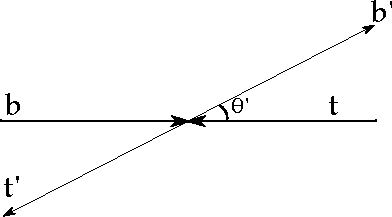
\includegraphics[width=0.4\columnwidth]{Rutherford-kin}
  \caption{Principskitse af impulserne i spredningsprocessen $b + t \rightarrow b' + t'$ set fra massemidtpunktssystemet.}
  \label{fig:ruther-kin}
  \vspace{-5mm}
\end{figure}

\Cref{fig:ruther-kin} skitserer den generelle spredningsproces
\begin{equation}
  \label{eq:spredning}
  b + t \rightarrow b' + t'.
\end{equation}

Den kinetiske energi af den udkommende partikel $b'$ i laboratoriesystemet (LAB) er givet ved
\begin{equation}
  \label{eq:udkommendeE}
  T_{b'} = \frac{1}{2}m_{b'} \mvec{V_{b'}}^{2} = \frac{1}{2}m_{b'}(V_{CM}^{2} + V_{b'}'^{2} +
  2V_{CM}V_{b'}'\cos \theta' ),
\end{equation}
hvor $V'$ angiver hastigheder i massemidtpunktssystemet (CM) og $\theta'$ vinklen mellem $b'$ og $t$.

Begrænser man sig til at se på Rutherfordspredning svarende til at $t' = t$ og $b' = b$, så må
$V_{b'}' = V_{b}'\,$, da Coulombkraften er konservativ. Denne kan bestemmes ud fra energien af strålen
$T_{b}$
\begin{equation}
  \label{eq:rutherUdCM}
  V_{b}' = \frac{\mu}{m_{b}}V_{b} = \frac{m_{t}}{m_{t}+m_{b}} \sqrt{\frac{2T_{b}}{m_{b}}},
\end{equation}
hvor $\mu$ betegner den reducerede masse. Indsættes denne i \cref{eq:udkommendeE} kan energien
udtrykkes ved kun én fri variabel
\begin{equation}
  \label{eq:rutherUdLab}
  T_{b} = T_{b} \frac{m_{b}}{(m_{t}+m_{b})^{2}} \Bigl(m_{b} + \frac{m_{t}^{2}}{m_{b}} + 2m_{t}\cos \theta'\Bigr).
\end{equation}
Rutherfordspredning i LAB-systemet vil derfor give anledning til et kontinuert spektrum givet ved
\cref{eq:rutherUdLab}. I CM er energien bestemt af energi- og impulsbevarelse og givet ved
\cref{eq:rutherUdCM}.

I det generelle tilfælde er det ikke så ligetil. Her udnyttes, at i CM skal
$\mvec{p_{t'}} + \mvec{p_{b'}} = \mvec{0}$. Endvidere skal den samlede energi af $b'$ og $t'$ være
lig energien $E_{CM}$, som ikke er bundet i massemidtpunktets bevægelse. Kombinerer man dette med
\cref{eq:rutherUdCM}, får man
\begin{equation}
  V_{b'}'^{2} = \frac{2E_{CM}}{m_{b'}(1+\frac{m_{b'}}{m_{t'}})}.
\end{equation}
Indsættes dette i \cref{eq:udkommendeE} er det muligt at bestemme energien af $b'$ i LAB-systemet ud
fra $\theta'$
\begin{align}
  T_{b'} = m_{b'} \Bigl(T_{b}&\frac{m_{b}}{(m_{t} + m_{b})^{2}} + \frac{E_{CM}}{m_{b'}(1+\frac{m_{b'}}{m_{t'}})} \notag\\
  &+ 2 \sqrt{T_{B}E_{CM} \frac{m_{b}}{m_{b'}}}\bigl[(m_{t} + m_{b})(1 + \frac{m_{b'}}{m_{t'}})^{1/2}\bigr]^{-1} \cos \theta'\Bigr).
  \label{eq:alphaUdLab}
\end{align}
Som ved Rutherfordspredning giver denne proces også anledning til et kontinuum i LAB-systemet og
en veldefineret energi i CM. 


\section{Data og databehandling}
\label{sec:ruther-data}

Databehandlingen af dette forsøg er simpel. For hver detekteret partikel bestemmes polarvinklen ud
fra hvilken detektor og forstrip, der rammes. For de firkantede detektorer er det også nødvendigt at
bestemme bagstrippen. Her findes den bagstrip, hvor energiforskellen er mindst mulig. Detektionen
afvises, hvis forskellen er større end 100\keV. Energien og polarvinklen tilføjes til et
2D-histogram.

\subsection{Tyndt folie}
\label{sec:tyndtfolie}

For at undgå andre processer end Rutherfordspredning er her benyttet et \SI[per-mode =
symbol]{4}{\micro\gram\per\cm\squared} kulstoffolie. Resultatet ses på \cref{fig:1072}, hvor
rækkevidden for protoner er anvendt. Som forventet fra teorien afhænger energien af den spredte
proton af spredningsvinklen og udgør et kontinuum i LAB-systemet.
\begin{figure}[htb]
  \centering
  \subbottom[LAB systemet]{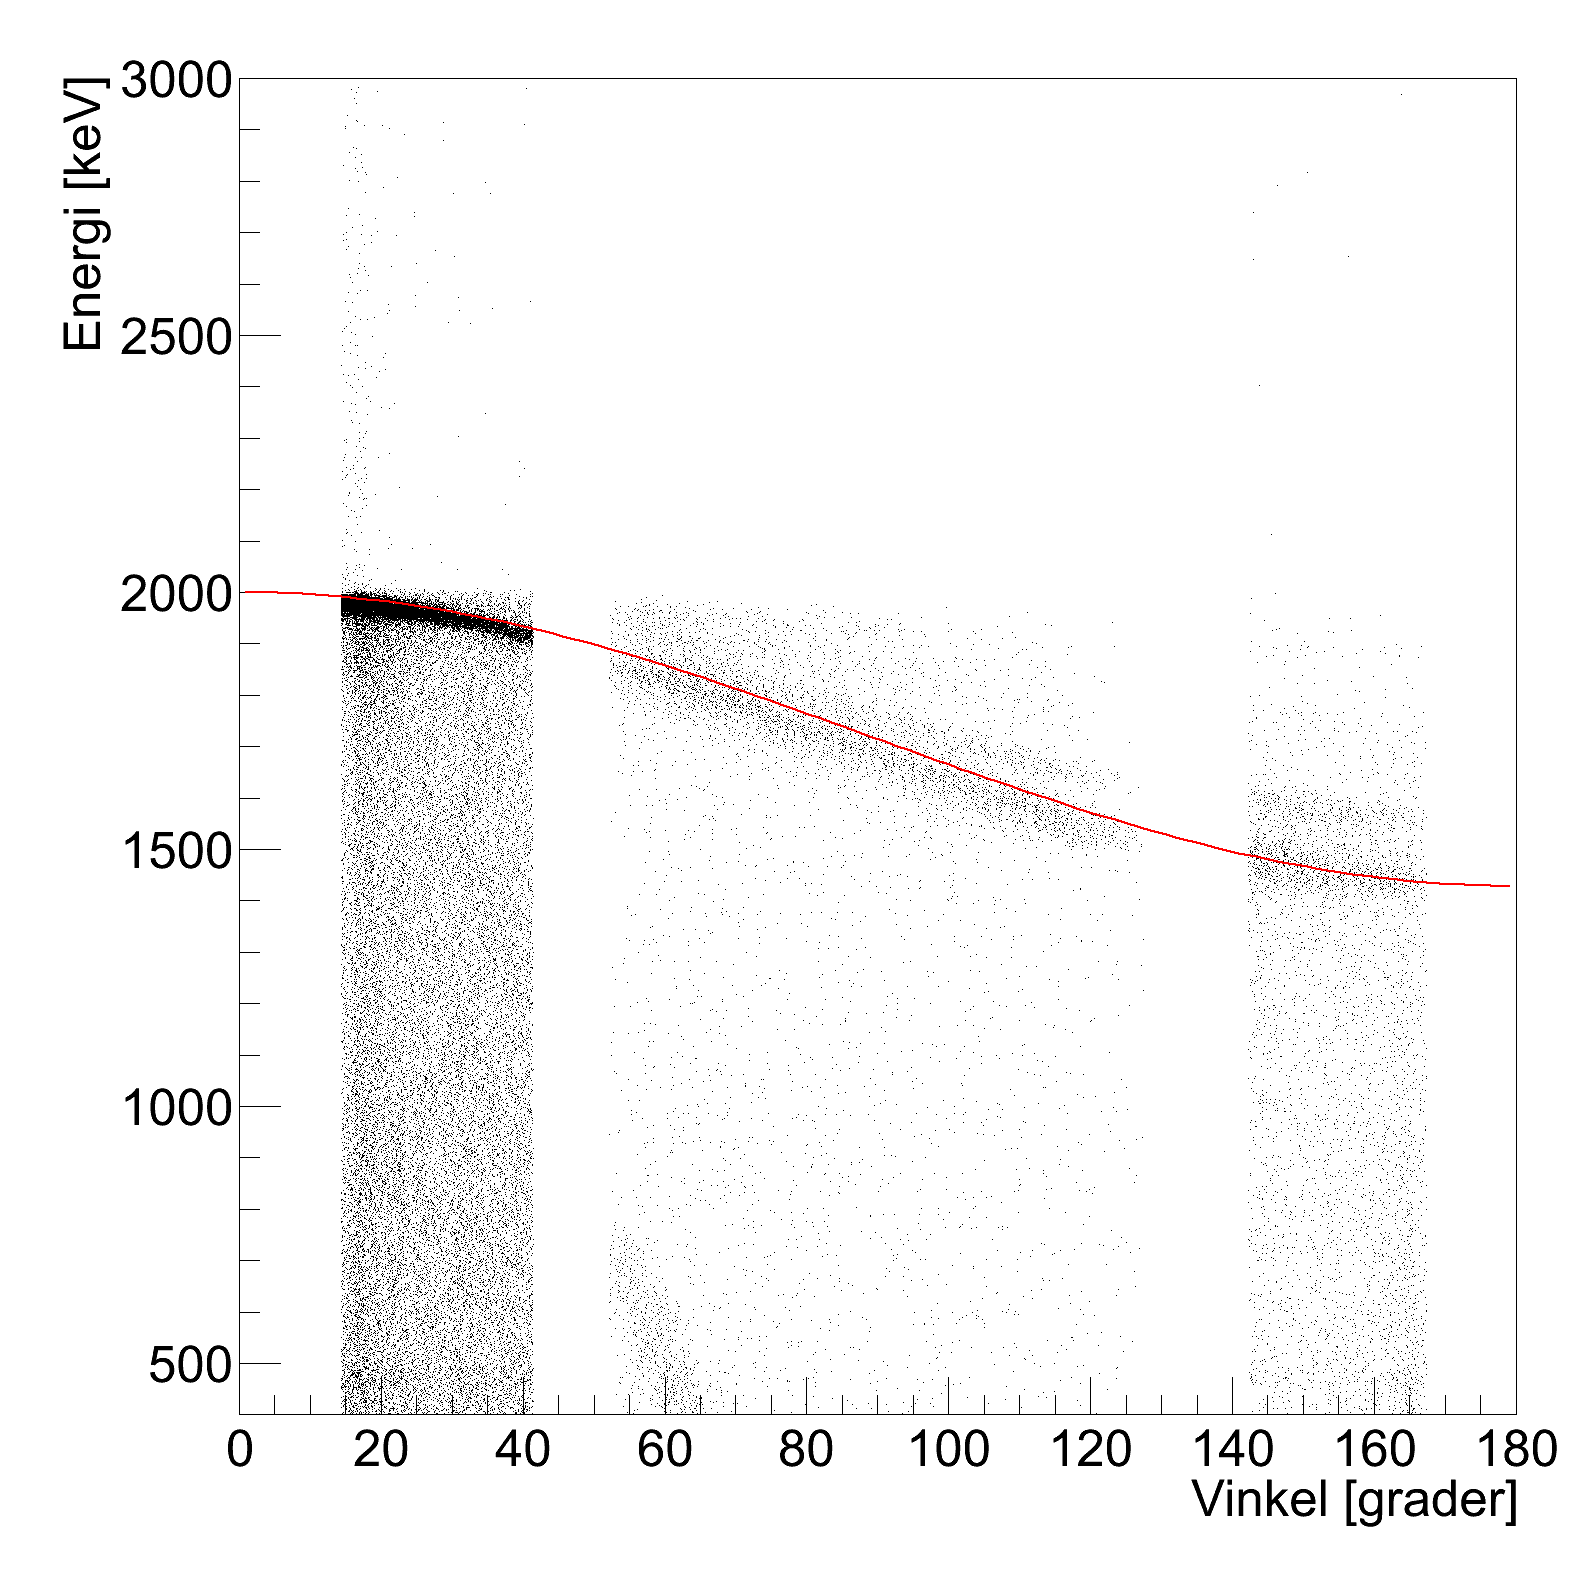
\includegraphics[width=0.49\columnwidth]{AngleEnergy1072-LABd}}%
  \hfill
  \subbottom[CM for protonen]{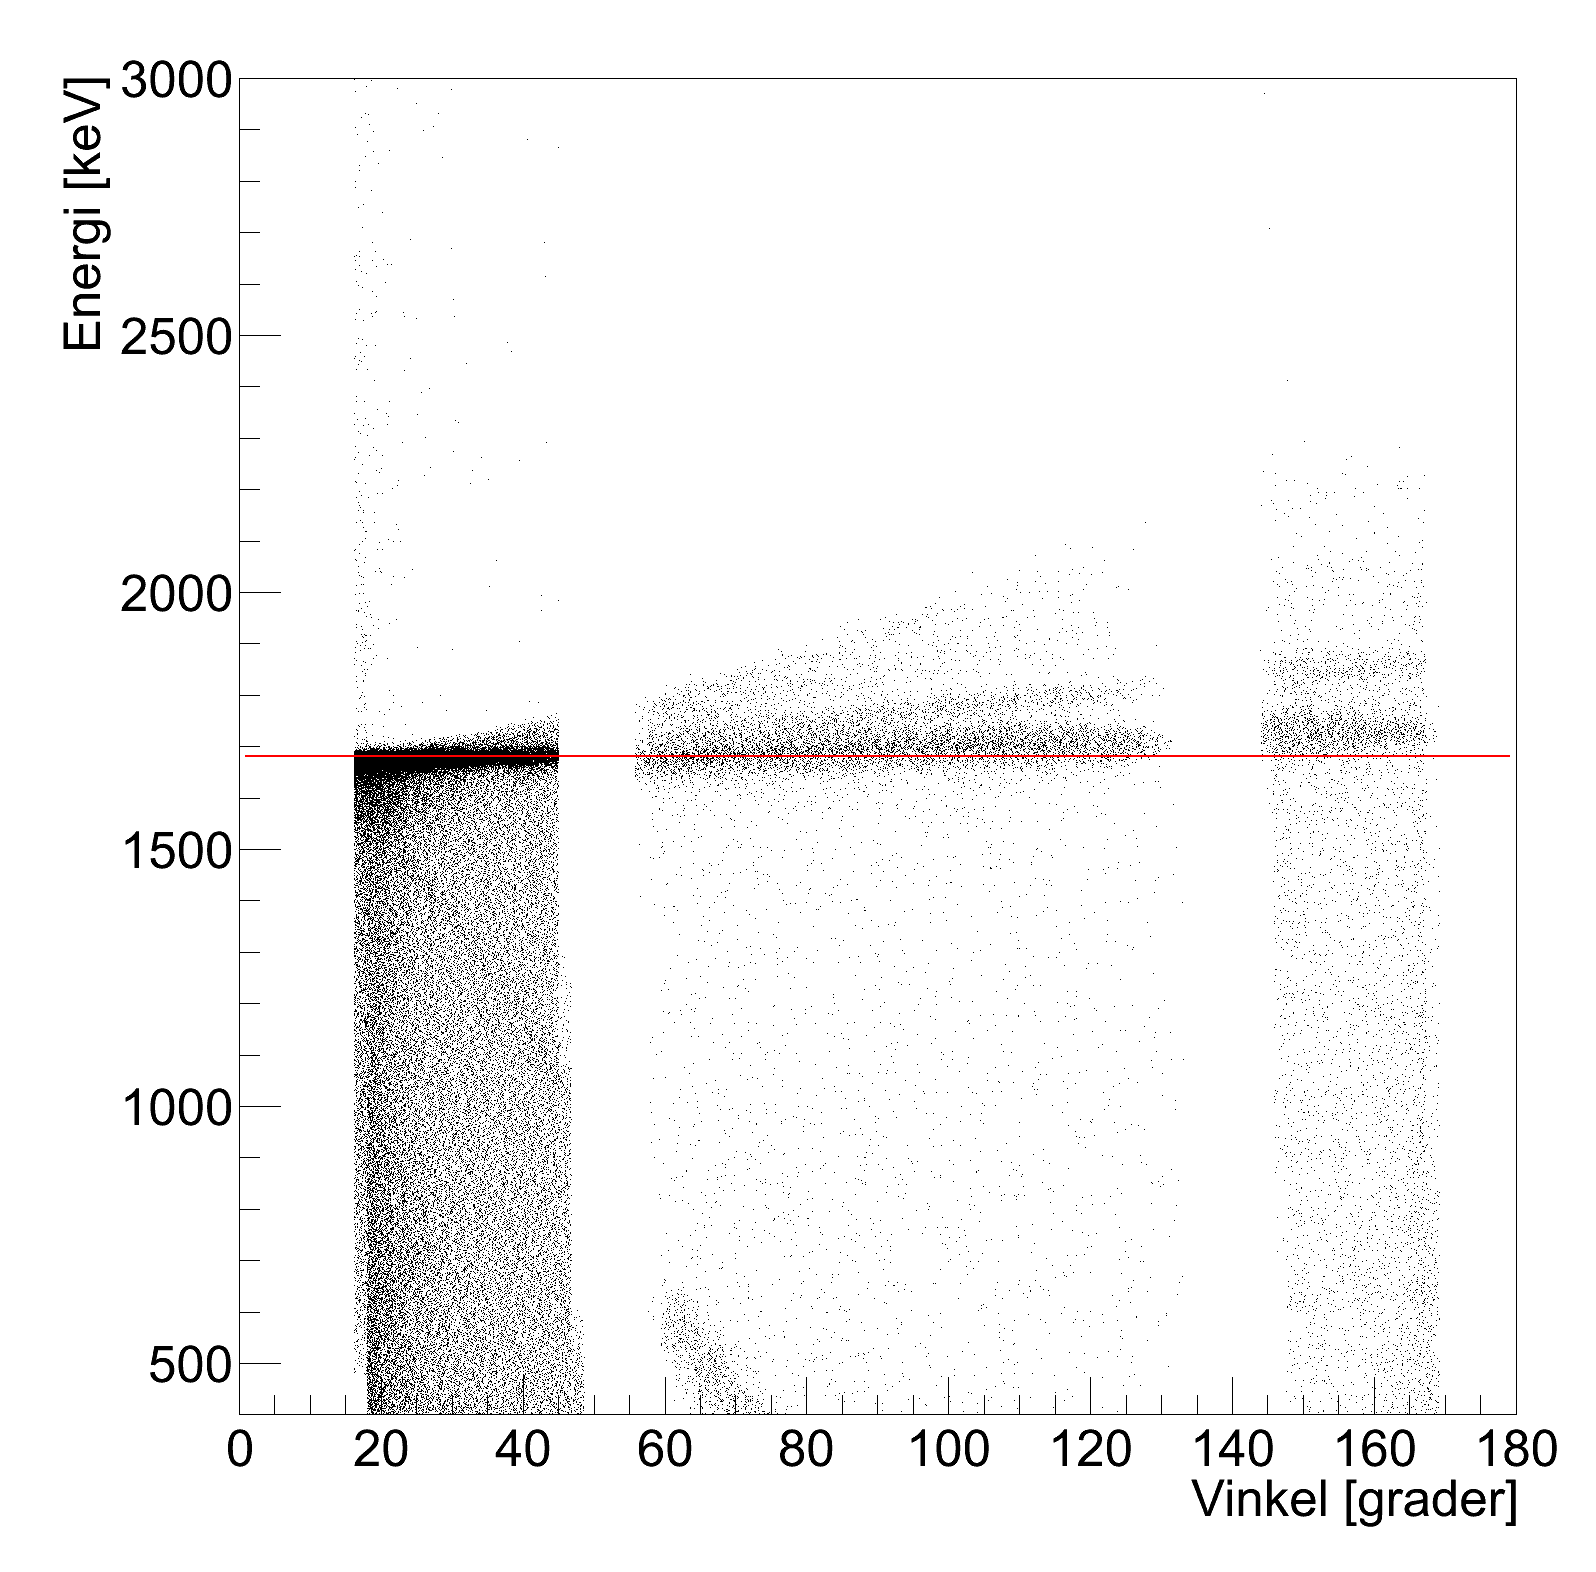
\includegraphics[width=0.49\columnwidth]{AngleEnergy1072-CMp}}%
  \caption{Antal tællinger som funktion af energi og vinkel for spredning af protoner på
    kulstof. Den røde linie er \cref{eq:rutherUdLab} med $m_{t} = m_{\!\!\Carb}$. Fra venstre mod
    højre ses data fra detektor 4, 1 og 3. Større tæthed angiver højere antal tællinger.}
  \label{fig:1072}
\end{figure}

\Cref{fig:1072}b viser det tilsvarende data, hvor der er transformeret til CM for protonen. Dette
viser, hvorledes energien af den udgående proton i CM med god tilnærmelse er en konstant. De
små usikkerheder for de runde detektorer skyldes primært usikkerheder på detektorernes
positioner.

Det lader også til, at energien fra de firkantede detektorer ligger en smule under kurven. Det kan
skyldes, at disse har et lille dødlag, der skal tages højde for. Dette er der dog ikke gjort i
denne opgave.

Data viser endvidere, at foliet ikke kun består af \Carb, men også af andre
grundstoffer. 

Her er både tale om et enkelt let grundstof, der ses under den røde linie samt tungere grundstoffer
over linien. Disse fordeler sig således, da de lette grundstoffer får en højere rekylenergi ved
sammenstød med protonen. Dette kan muligvis skyldes vand på foliet. 

\subsection{\Bor folie}
\label{sec:tykt-folie}

Her ses på data fra protonbeskydning af det \Bor-folie, som er benyttet gennem resten af
eksperimentet. Her forventes ud over Rutherfordspredning også reaktionen
$p + \Bor \rightarrow \Carb*$. Dette kulstof er ustabilt og vil henfalde igen. I
\cref{cha:sekventielt-henfald} vil der blive redegjort for henfaldsprocessen i detaljer, specifikt
udledes i \cref{sec:tilstand} et udtryk for energien i CM
\begin{equation}
  E_{CM} = \frac{11}{12} T_{p} + Q = \frac{11}{12} T_{p} + m_{p} + m_{\!\!\Bor} - m_{\alpha} - m_{\Be},
\end{equation}
hvor det første led følger af $V_{CM} = \mu V_{b} / m_{b}$. 

\Cref{fig:1077} viser data og den teoretiske kurve givet ved \cref{eq:alphaUdLab}. Her er anvendt
rækkevidden for $\alpha$-partikler, hvilket er årsagen til, at Rutherfordlinien passer så
dårligt. Rutherfordlinien i de runde detektorer krummer opad mod områderne svarende til store
detektorvinkler. Dette skyldes overkompensation for dødlaget.  Den samme effekt ses også i $\alpha$-linien
i CM, hvilket tyder på, at dødlaget er tyndere end de estimerede \SI{0,6}{\um}.

På trods af disse små effekter stemmer spektret fint overens med de kinematiske kurver, hvilket
indikerer, at \Carb* kan foretage $\alpha$-henfald.

Det noteres, at \Bor foliet indeholder flere urenheder end bagbeklædningen.
\begin{figure}[ht]
  \fxfatal{Her skal tilføjes linier til CM.}
  \centering
  \subbottom[LAB systemet]{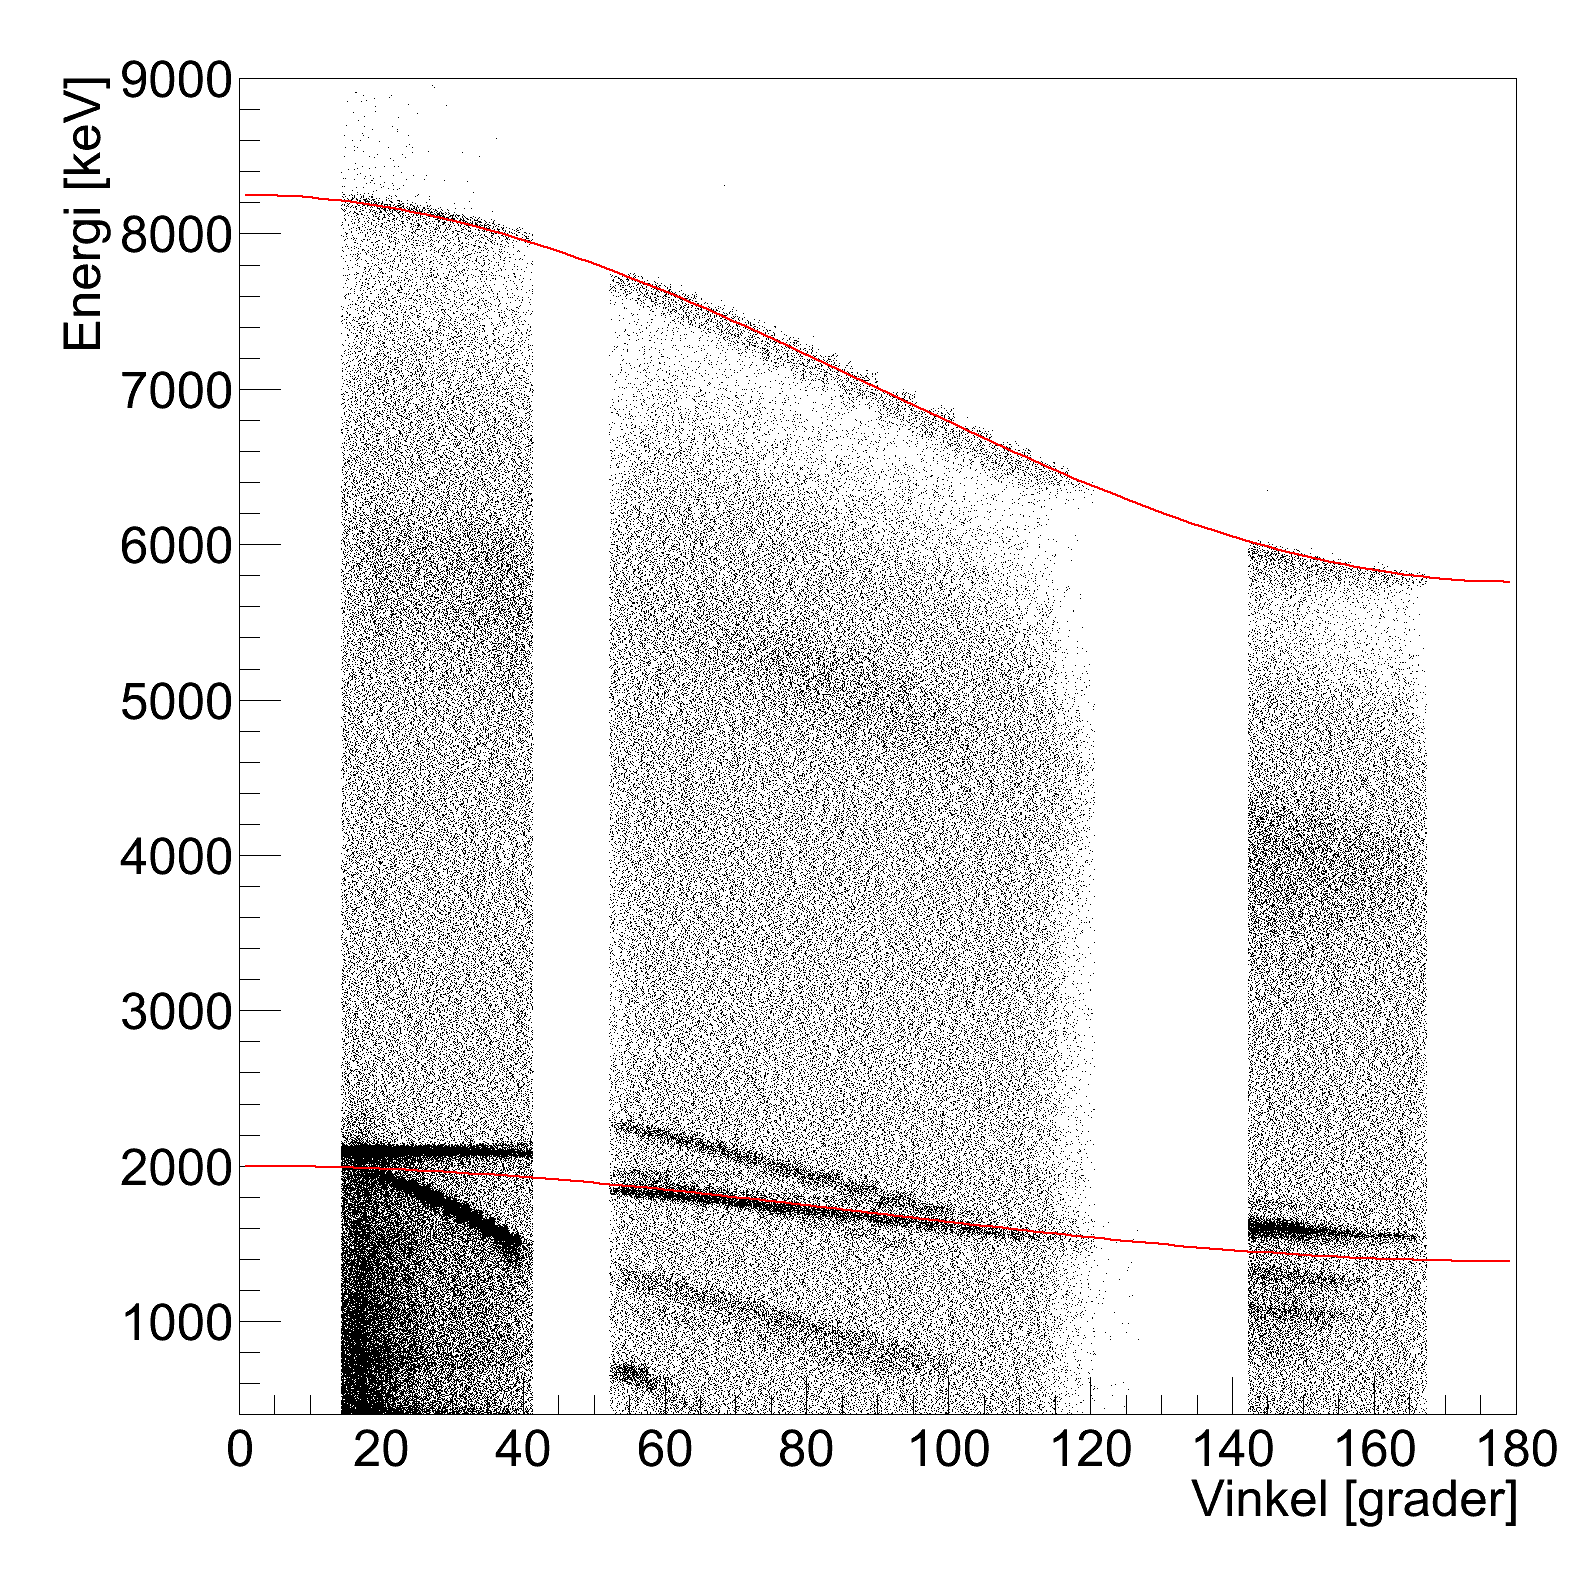
\includegraphics[width=0.49\columnwidth]{AngleEnergy1077-LABd}}%
  \hfill
  \subbottom[CM for $\alpha$-partiklen]{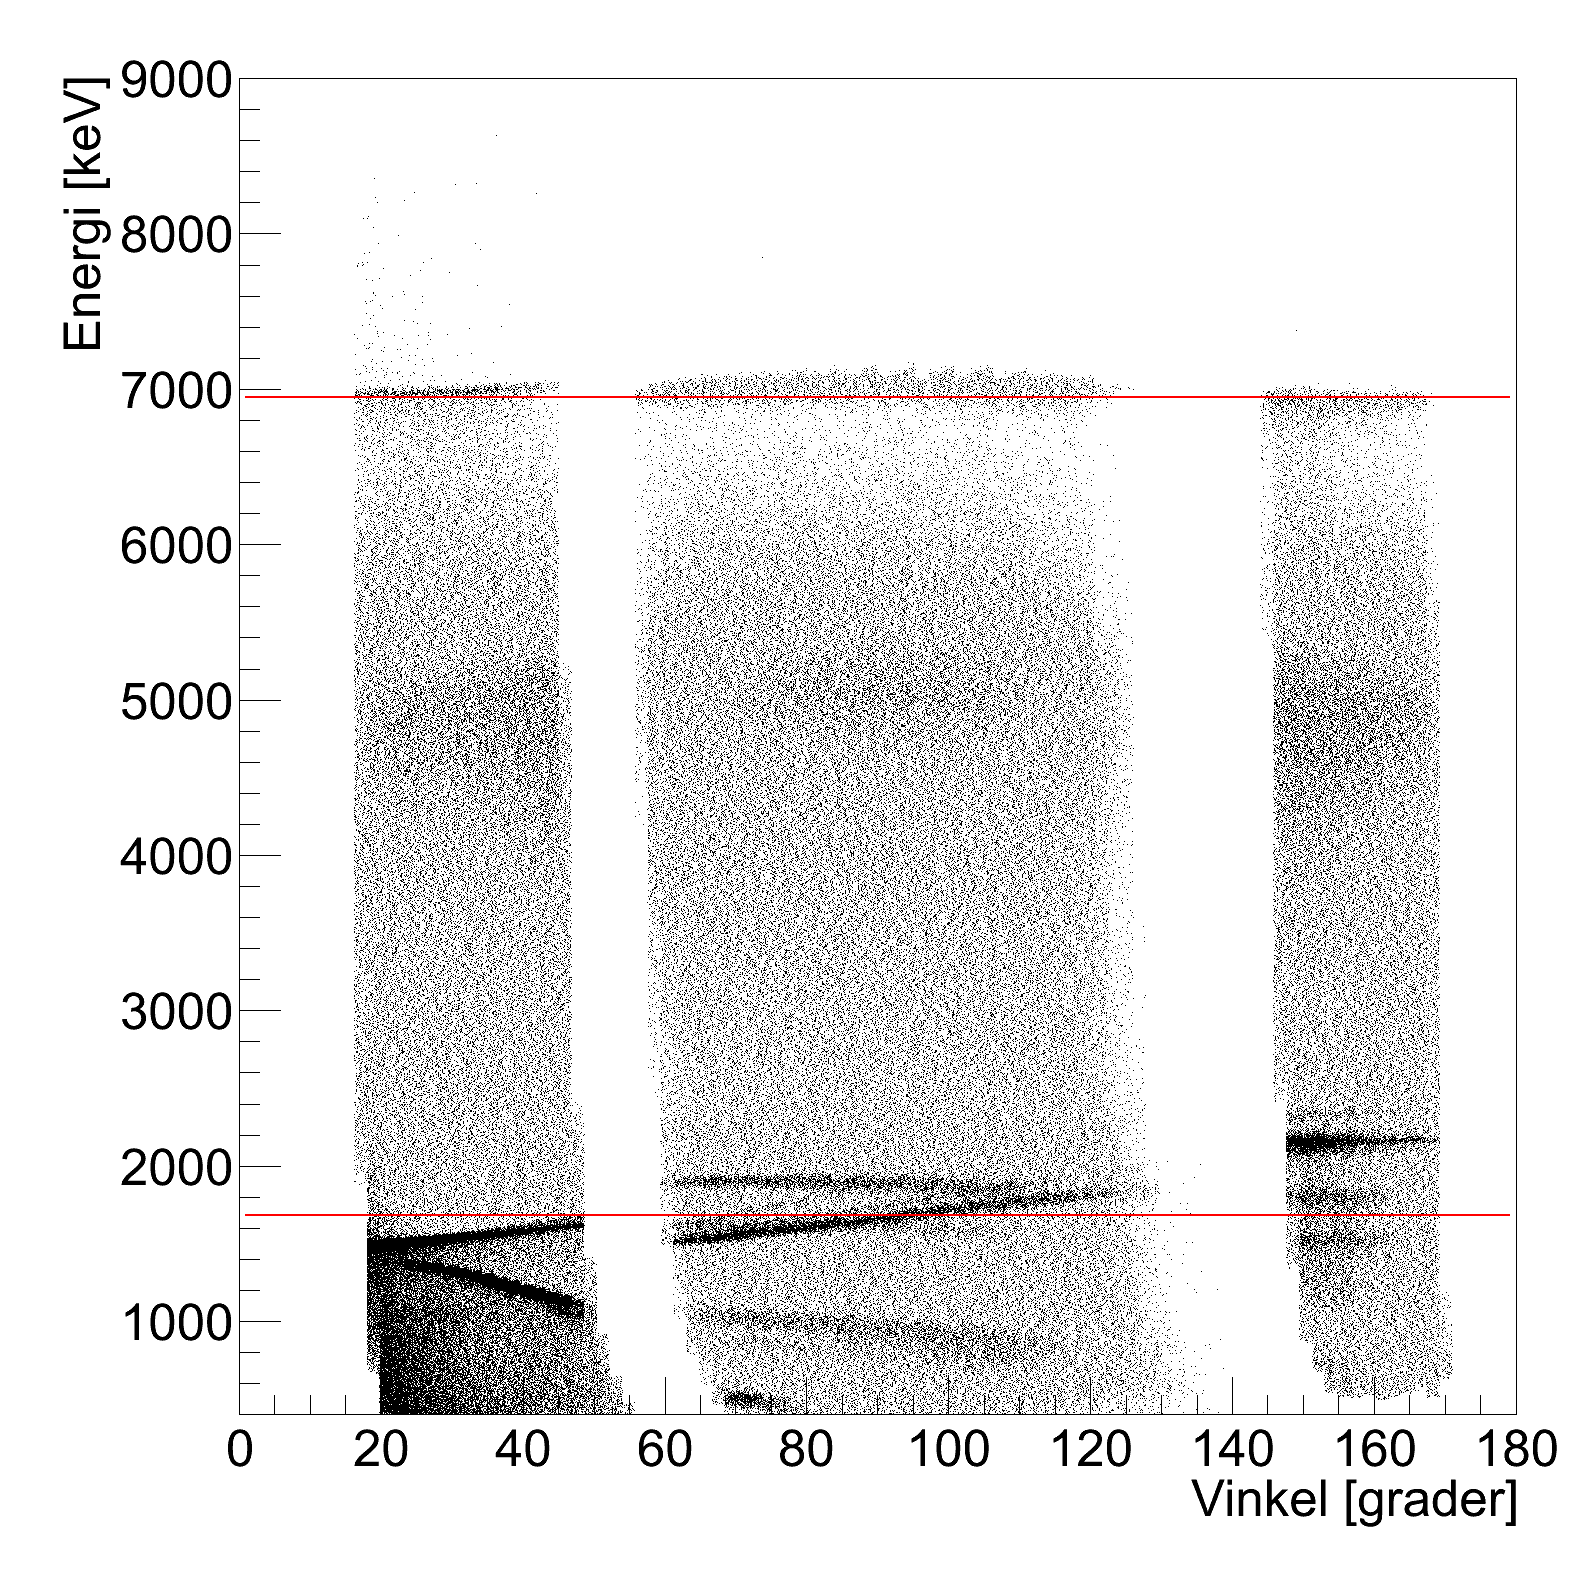
\includegraphics[width=0.49\columnwidth]{AngleEnergy1077-CMa}}%
  \caption{Antal tællinger som funktion af energi og vinkel for spredning af protoner på \Be. Den
    øverste røde linie er \cref{eq:alphaUdLab} og den nederste er \cref{eq:rutherUdLab}. I begge
    tilfælde er $m_{t} = m_{\!\!\Bor}$. Fra venstre mod højre ses data fra detektor 4, 1 og
    3. Større densitet angiver højere antal tællinger.}
  \label{fig:1077}
\end{figure}

\section{Resultater}
\label{sec:ruther-konklusion}
Det er vist, at de eksperimentielt opnåede kinematiske kurver stemmer godt overens med de
teoretiske. Der er observeret afvigelser, der indikerer, at tykkelsen af dødlaget for S3
detektorerne er overvurderet en smule og W1 detektorerne muligvis har et lille dødlag. Størrelsen af
disse afvigelser er dog små. Kalibreringen kan derfor benyttes til den videre analyse.







